\chapter{Results Analysis}
\label{chap:results}

This chapter presents a comprehensive quantitative and qualitative evaluation of the proposed passive face anti-spoofing and biometric attendance framework. Experiments progress systematically from optimization convergence and standardized ISO/IEC 30107-3 frame-level error rates on the subject-disjoint \texttt{Cam4K} benchmark to video-level aggregation, cross-camera retention, CPU/HTTP latency profiling, attendance threshold calibration, failure-mode inspection, and multi-factor ablation studies.

\section{Experimental Setup}
\label{sec:experimental_setup}

All evaluations were executed on the CPU workstation detailed in Table~\ref{tab:software_stack} (AMD Ryzen~7 6800H, $8$~cores / $16$~threads, $16.0$~GB RAM, Windows~11, Python~3.11.9, TensorFlow~2.19.0, LiteRT XNNPACK, OpenCV~4.11.0). No discrete GPU acceleration was utilized during runtime or latency benchmarking, mirroring target edge attendance deployments.

To assess real-world behavior without optimistic bias, models were evaluated across four distinct operational granularities referencing the partitions established in Chapter~\ref{chap:data_processing}:
\begin{enumerate}
    \item \textbf{Person-disjoint frame evaluation:} Every extracted $32\times32$ facial crop in the unaugmented \texttt{Cam4K} validation ($5{,}015$ crops, $14$ videos) and unseen test ($4{,}811$ crops, $14$ videos) partitions---as well as the $4{,}856$-crop test split of the $89$-video Merged Multi-Source Benchmark and $600$ external laptop-webcam crops---was scored independently at decision threshold $0.50$.
    \item \textbf{Video-level probability aggregation:} Frame-wise softmax probabilities $[P_{\text{fake}}, P_{\text{real}}]$ were averaged across each full video recording ($14$ \texttt{Cam4K} test videos; $16$ Cohort~IIa multi-subject test videos). On Cohort~IIa, statistical uncertainty of video-level gains over the pre-retrain baseline was quantified via $2{,}000$-iteration paired bootstrap resampling (\texttt{seed = 42}).
    \item \textbf{Continuous session replay:} Sixteen unseen test videos were streamed sequentially through the full end-to-end \texttt{Pipeline} ($12$~seconds per video at $5$~FPS, $942$ total frames) under \texttt{TemporalDecision} hysteresis to measure active decision coverage versus false-authorization count.
    \item \textbf{Microservice and attendance integration profiling:} Single-crop LiteRT latency ($200$ timed iterations following $20$ warmup passes), Waitress HTTP loopback latency, and \texttt{ChamCong\_FaceID} leave-one-video-out / leave-one-person-out cosine threshold sweeps were benchmarked directly on the host CPU.
\end{enumerate}

\section{Evaluation Strategy}
\label{sec:evaluation_strategy}

Standard classification metrics are reported alongside domain-specific biometric security criteria. For each class $c \in \{\text{fake}, \text{real}\}$ with true positives $\text{TP}_c$, false positives $\text{FP}_c$, and false negatives $\text{FN}_c$, class-wise Precision, Recall, $F_1$-score, and unweighted Macro-$F_1$ are computed as shown in Equation~\eqref{eq:macro_f1}:
\begin{equation}
\label{eq:macro_f1}
\begin{aligned}
    \text{Precision}_c &= \frac{\text{TP}_c}{\text{TP}_c + \text{FP}_c}, \qquad
    \text{Recall}_c = \frac{\text{TP}_c}{\text{TP}_c + \text{FN}_c}, \\
    F_{1,c} &= \frac{2\,\text{Precision}_c\,\text{Recall}_c}{\text{Precision}_c + \text{Recall}_c}, \qquad
    \text{Macro-}F_1 = \frac{F_{1,\text{fake}} + F_{1,\text{real}}}{2}.
\end{aligned}
\end{equation}

Biometric vulnerability is governed by the ISO/IEC 30107-3~\cite{iso30107_3} triad defined in Equation~\eqref{eq:iso_metrics}: $\text{APCER}$ (fraction of presentation attacks falsely accepted as \texttt{real}), $\text{BPCER}$ (fraction of bona fide users falsely rejected as \texttt{fake}), and their arithmetic mean $\text{ACER}$. In biometric attendance gating, elevated $\text{APCER}$ represents a direct security breach (fraudulent check-in), whereas elevated $\text{BPCER}$ causes user friction requiring a second scan.

For stateful multi-frame sessions ($N_{\text{total}}$ streamed frames) where fail-closed gates may abstain via \texttt{checking}, \texttt{adjust}, or \texttt{uncertain} states, letting $N_{\text{correct}}$ and $N_{\text{wrong}}$ denote frames emitting committed \texttt{real}/\texttt{fake} verdicts that match or contradict ground truth, Session Coverage and Committed Error Rate are defined in Equation~\eqref{eq:session_coverage}:
\begin{equation}
\label{eq:session_coverage}
    \text{Coverage} = \frac{N_{\text{correct}} + N_{\text{wrong}}}{N_{\text{total}}}, \qquad
    \text{Error}_{\text{committed}} = \frac{N_{\text{wrong}}}{\max(N_{\text{correct}} + N_{\text{wrong}}, 1)}.
\end{equation}

\section{Quantitative Results}
\label{sec:quantitative_results}

\subsection{Optimization Convergence on \texttt{Cam4K}}

Figure~\ref{fig:learning_curves} plots categorical cross-entropy loss and frame-level classification accuracy across all $18$ epochs of Algorithm~\ref{alg:training} on the \texttt{Cam4K} benchmark (\texttt{outputs/cam4k-restore/history.json}).

\begin{figure}[htbp]
\centering
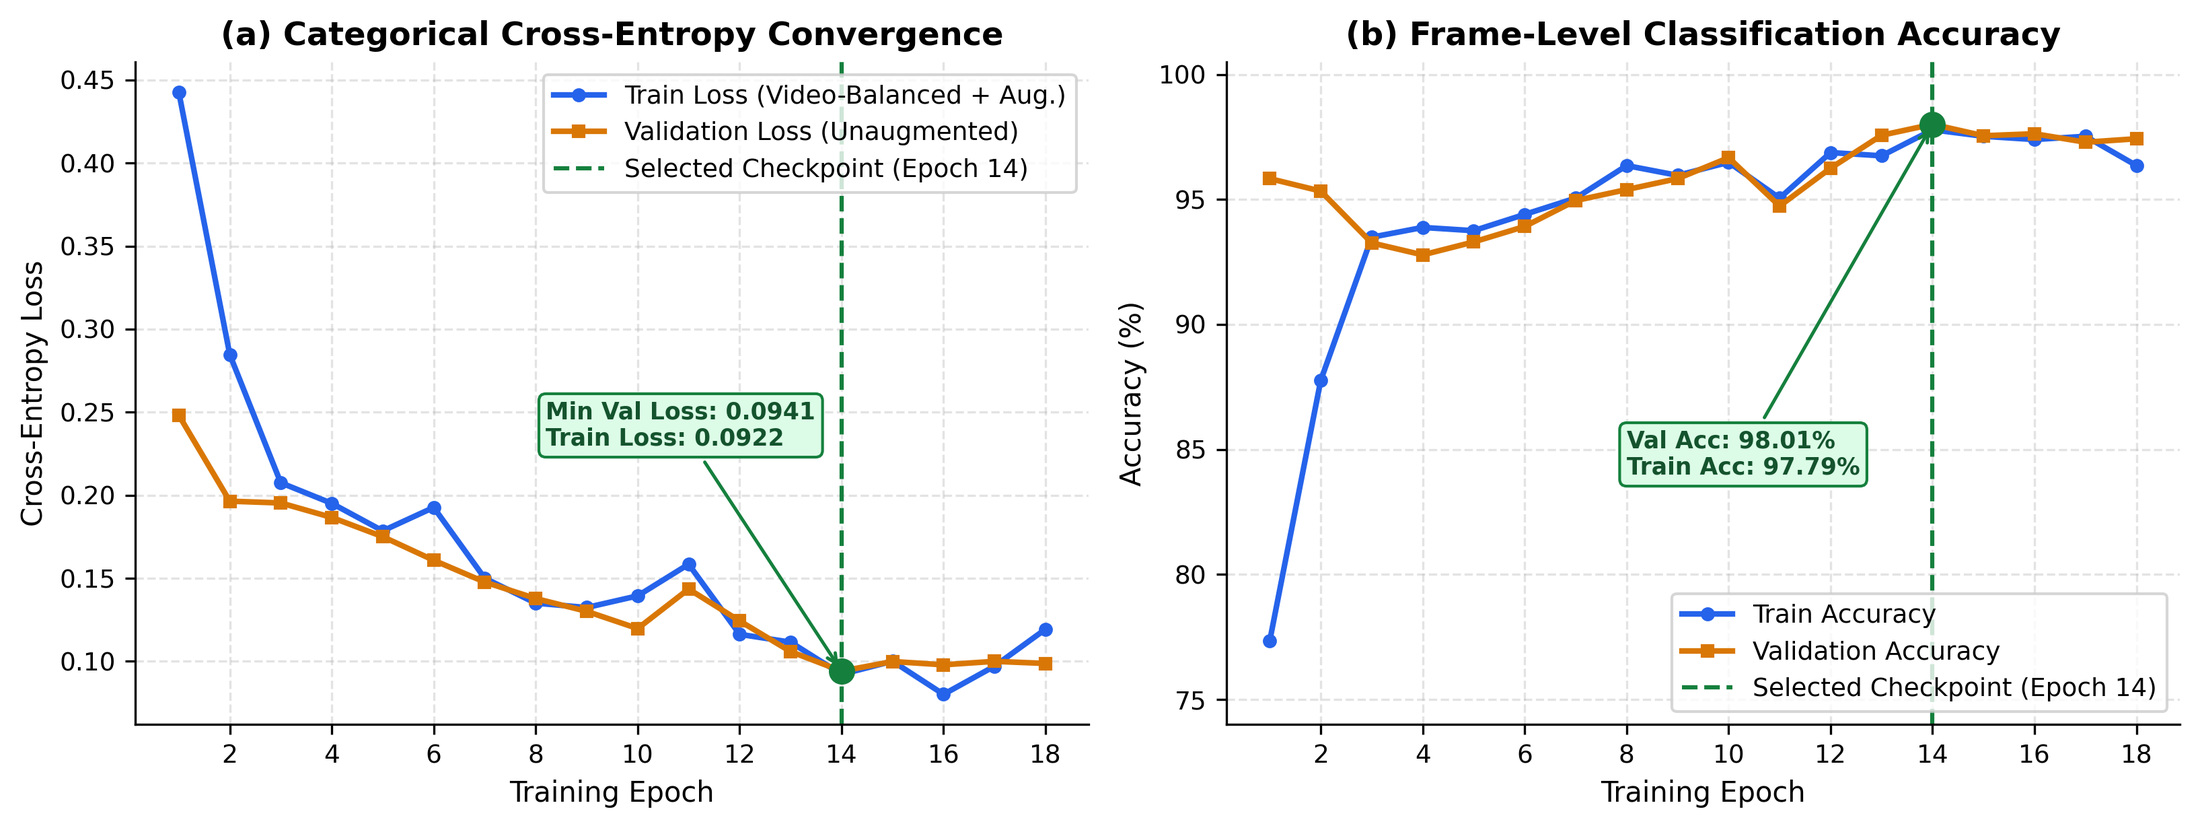
\includegraphics[width=0.98\textwidth]{Images/fig_cam4k_learning_curves.jpg}
\caption{Training and validation convergence curves on the person-disjoint \texttt{Cam4K} corpus over $18$ epochs: (a) categorical cross-entropy loss; (b) frame-level accuracy, marking the optimal validation checkpoint at Epoch~$14$.}
\label{fig:learning_curves}
\end{figure}

During Epoch~$1$, training loss starts at $0.4437$ ($77.38\%$ accuracy) under active geometric and white-balance augmentation, whereas unaugmented validation loss immediately reaches $0.2484$ ($95.85\%$ accuracy) because the frozen convolutional backbone already encodes multi-source surface primitives and validation crops contain no stochastic distortion. Both trajectories decrease monotonically without divergence through Epoch~$14$, where validation loss achieves its global minimum of $\mathcal{L}_{\text{val}} = 0.0941$ ($98.01\%$ validation accuracy) alongside $\mathcal{L}_{\text{train}} = 0.0922$ ($97.79\%$ training accuracy). The negligible generalization gap ($\Delta\mathcal{L} = 0.0019$) confirms that freezing early convolutional filters and regularizing the $512$-unit head eliminated overfitting to training identities. Applying WiSE-FT head interpolation ($\lambda = 0.75$) on top of the Epoch~$14$ checkpoint further lifted unaugmented validation accuracy from $98.01\%$ to $98.88\%$.

\subsection{Frame-Level Classification and ISO/IEC 30107-3 Metrics}

Table~\ref{tab:cam4k_metrics} reports the complete classification and PAD error breakdown of the final aligned \texttt{LivenessNet} artifact (\texttt{liveness\_cam4k.h5} / \texttt{.tflite}) on both the $5{,}015$-frame validation partition and the strictly unseen $4{,}811$-frame test partition. Figure~\ref{fig:confusion_matrices} visualizes the corresponding confusion matrices.

\begin{table}[htbp]
\centering
\caption{Quantitative frame-level and video-level performance of aligned \texttt{LivenessNet} on the person-disjoint \texttt{Cam4K} benchmark.}
\label{tab:cam4k_metrics}
\small
\begin{tabular}{L{4.8cm}R{2.3cm}R{2.3cm}R{3.6cm}}
\toprule
\textbf{Evaluation Metric} & \textbf{Validation Set} & \textbf{Unseen Test Set} & \textbf{ISO / Security Target} \\
\midrule
Evaluated Videos (Person-Disjoint) & $14$ ($7$R / $7$F) & $14$ ($7$R / $7$F) & Zero subject overlap \\
Evaluated $32\times32$ Face Crops & $5{,}015$ & $4{,}811$ & Unaugmented frames \\
\midrule
Class \texttt{fake} Precision (\%) & $98.14$ & $\mathbf{99.87}$ & High confidence on flags \\
Class \texttt{fake} Recall / TNR (\%) & $99.69$ & $\mathbf{96.24}$ & $100\% - \text{APCER}$ \\
Class \texttt{fake} $F_1$-Score (\%) & $98.91$ & $\mathbf{98.02}$ & Balanced spoof detection \\
\midrule
Class \texttt{real} Precision (\%) & $99.67$ & $\mathbf{96.48}$ & Low false-accept leakage \\
Class \texttt{real} Recall / TPR (\%) & $98.06$ & $\mathbf{99.88}$ & $100\% - \text{BPCER}$ \\
Class \texttt{real} $F_1$-Score (\%) & $98.86$ & $\mathbf{98.15}$ & Balanced live acceptance \\
\midrule
Overall Frame Accuracy (\%) & $98.88$ & $\mathbf{98.09}$ & --- \\
Macro Precision / Macro Recall (\%) & $98.91$ / $98.87$ & $\mathbf{98.18}$ / $\mathbf{98.06}$ & --- \\
Macro $F_1$-Score (\%) & $98.88$ & $\mathbf{98.09}$ & --- \\
\midrule
$\text{APCER}$ --- Spoof False Accept (\%) & $0.31$ ($8/2546$) & $\mathbf{3.76}$ ($89/2365$) & Minimize security breach \\
$\text{BPCER}$ --- Live False Reject (\%) & $1.94$ ($48/2469$) & $\mathbf{0.12}$ ($3/2446$) & Minimize check-in friction \\
$\text{ACER}$ --- Average PAD Error (\%) & $1.13$ & $\mathbf{1.94}$ & Objective $< 2.50\%$ met \\
\midrule
Video-Level Mean-Prob Accuracy (\%) & $\mathbf{100.00}$ ($14/14$) & $\mathbf{100.00}$ ($14/14$) & Objective $> 95.0\%$ met \\
\bottomrule
\end{tabular}
\end{table}

\begin{figure}[htbp]
\centering
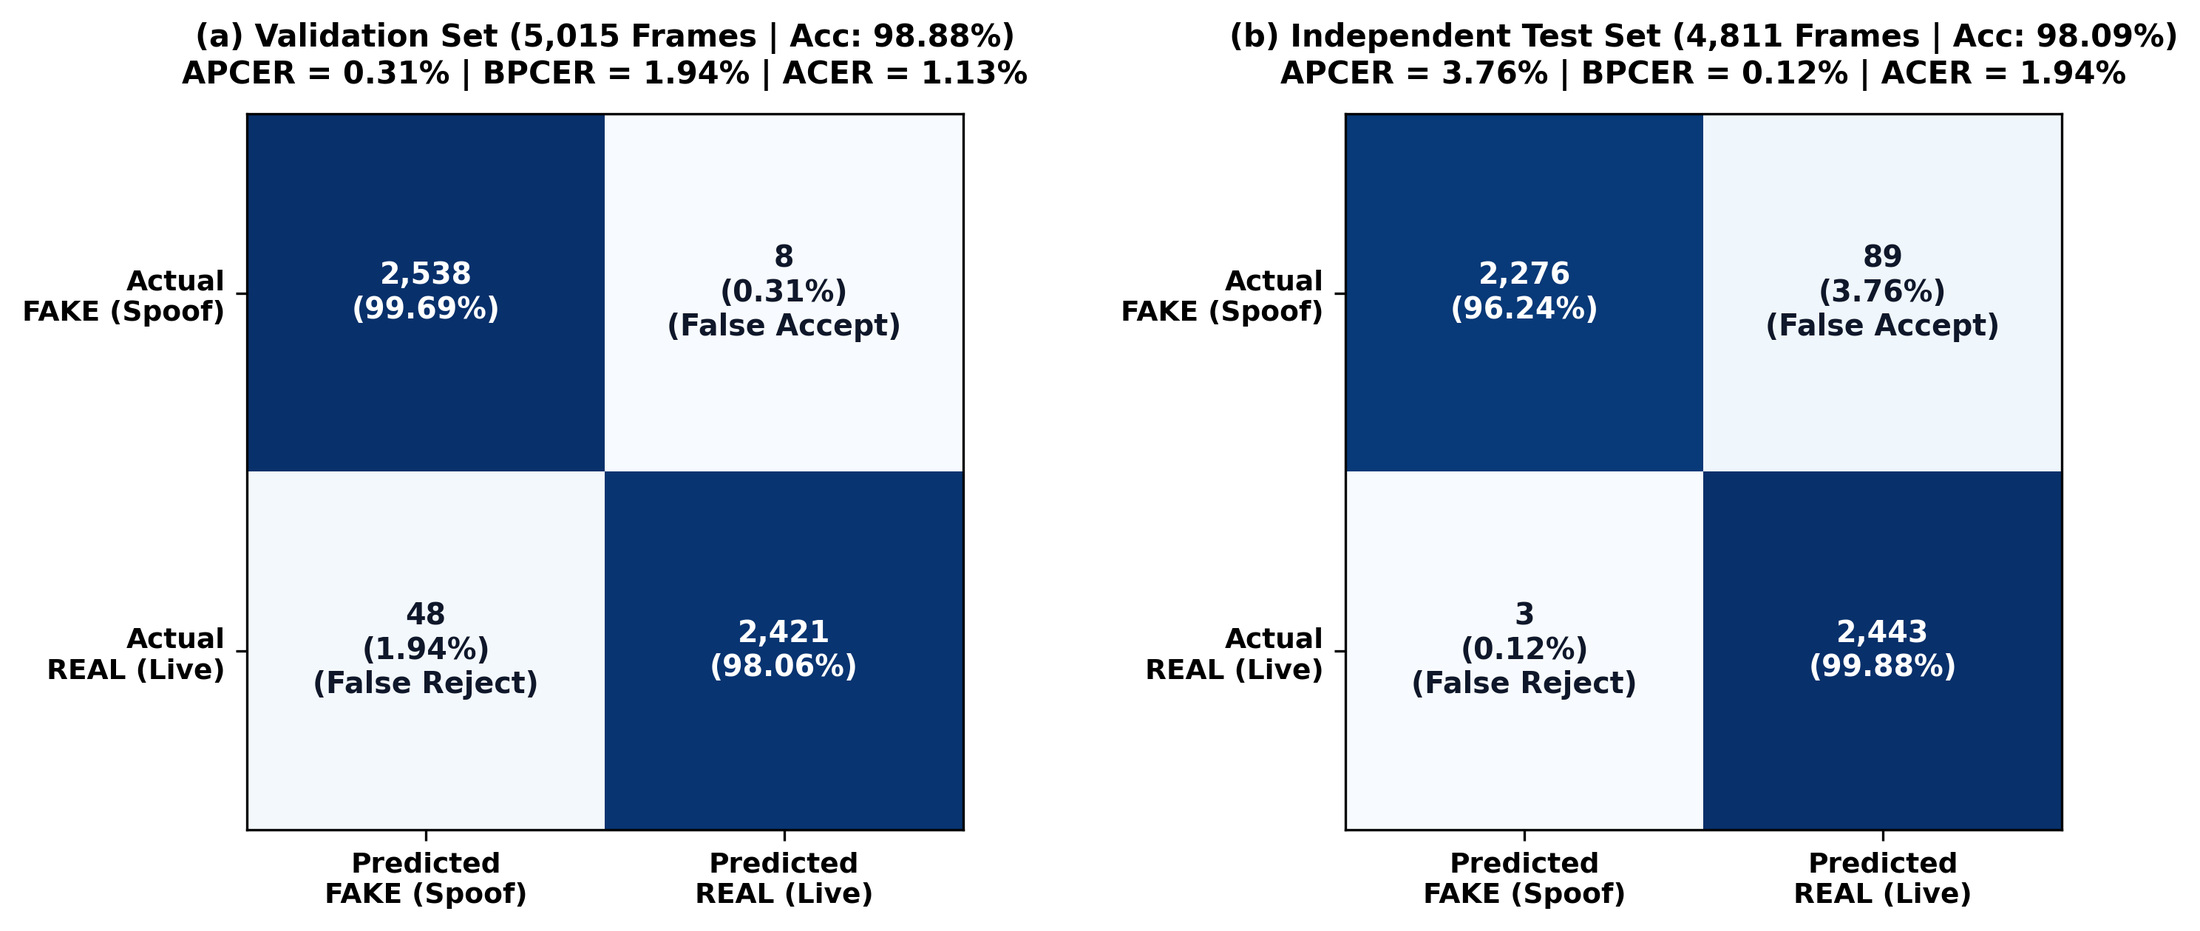
\includegraphics[width=0.98\textwidth]{Images/fig_confusion_matrices.jpg}
\caption{Frame-level confusion matrices on \texttt{Cam4K}: (a) validation partition ($5{,}015$ crops, $\text{ACER}=1.13\%$); (b) independent subject-disjoint test partition ($4{,}811$ crops, $\text{ACER}=1.94\%$).}
\label{fig:confusion_matrices}
\end{figure}

On the $4{,}811$ unseen test crops, the classifier correctly labels $4{,}719$ frames ($98.09\%$ overall accuracy, $98.09\%$ Macro-$F_1$), achieving $\text{ACER} = 1.94\%$---well within the $<2.50\%$ target specified in Chapter~\ref{chap:introduction}. Notably, bona fide false rejections are virtually eliminated on unseen test subjects ($\text{BPCER} = 0.12\%$, only $3$ frames misclassified out of $2{,}446$ live crops, yielding $99.87\%$ \texttt{fake} precision). Meanwhile, $2{,}276$ of $2{,}365$ spoof frames are rejected at the raw single-frame level ($\text{APCER} = 3.76\%$), before any multi-frame temporal smoothing is applied.

\subsection{Video-Level Aggregation and Cross-Camera Generalization}

In operational attendance check-ins, a camera observes a continuous stream of frames rather than an isolated $32\times32$ crop. Figure~\ref{fig:video_probabilities} and Table~\ref{tab:video_breakdown} present the video-level mean probabilities across all $14$ unseen test videos in \texttt{Cam4K}.

\begin{figure}[htbp]
\centering
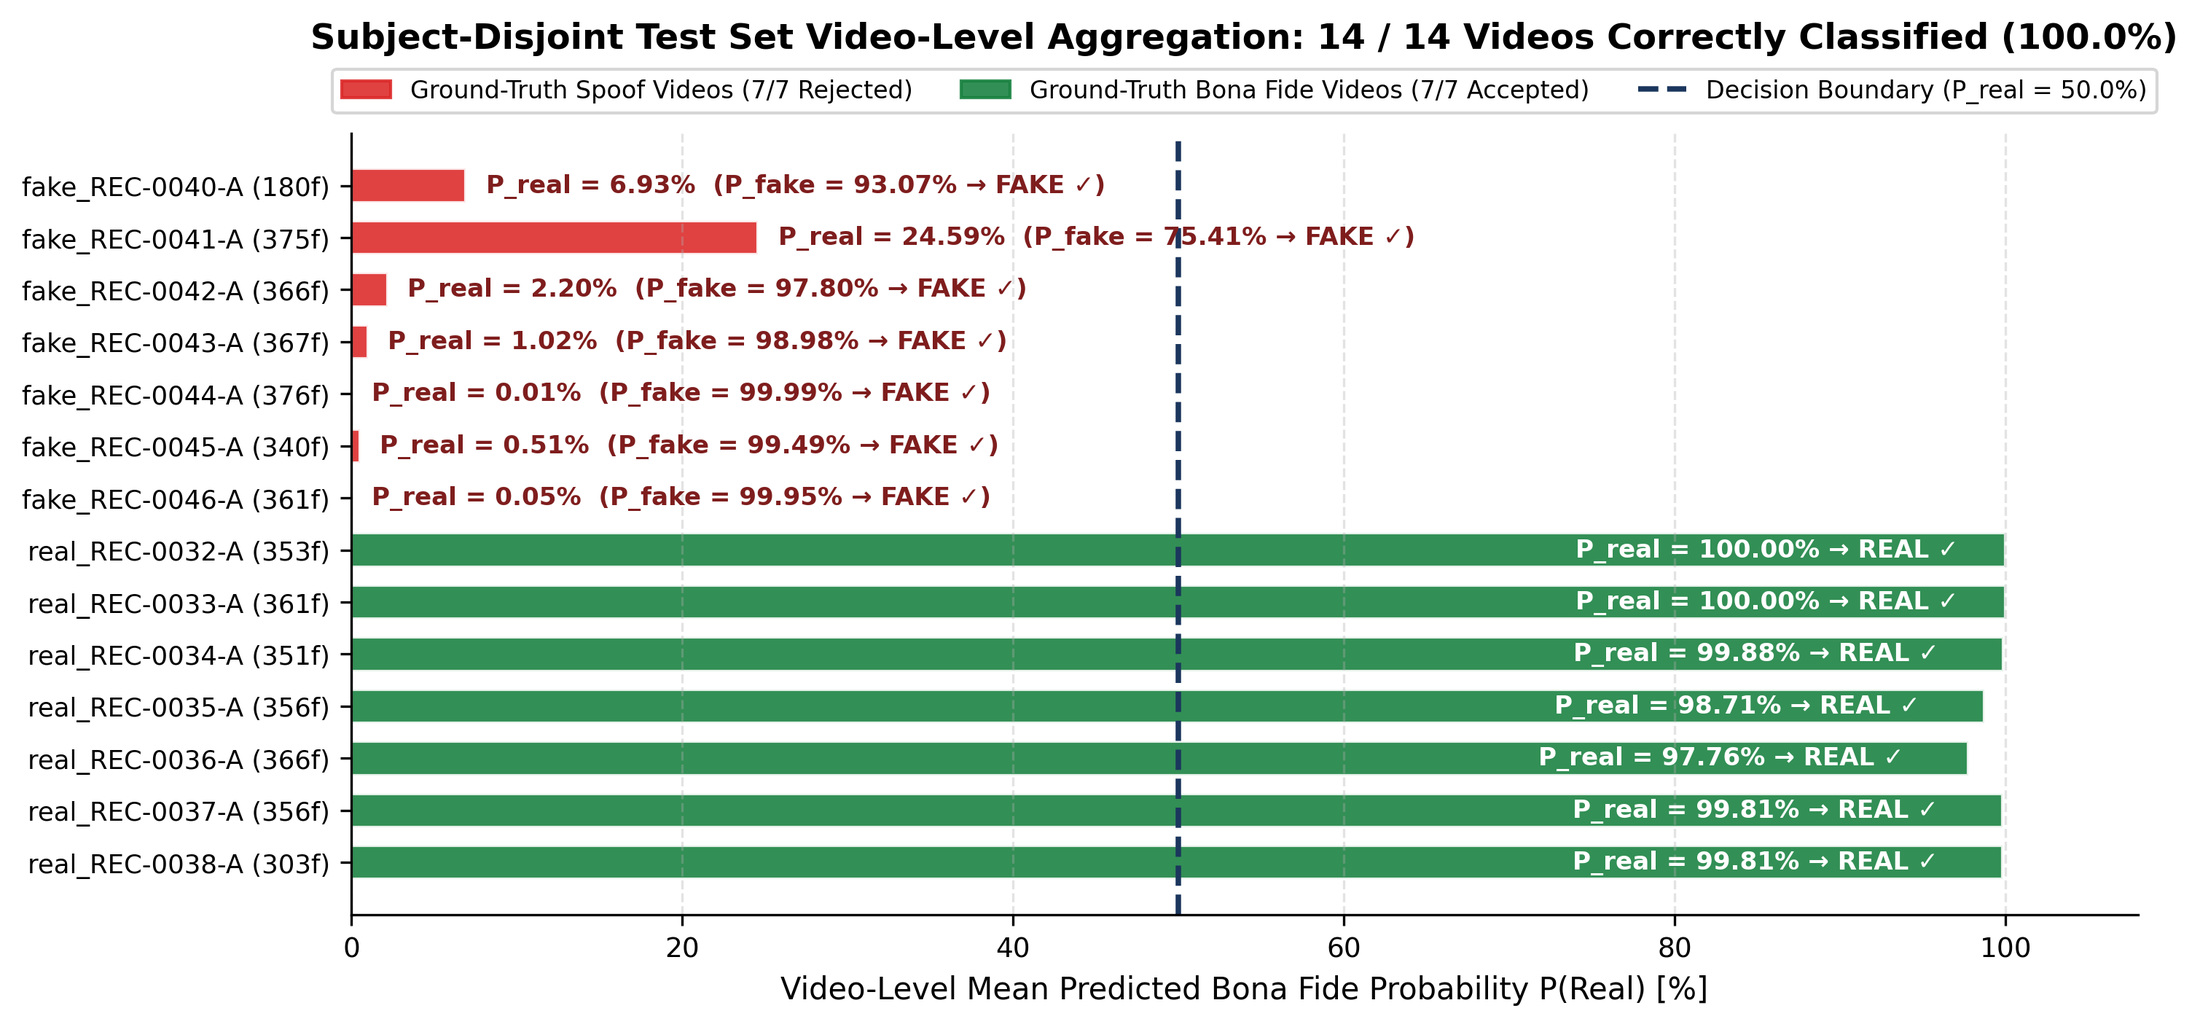
\includegraphics[width=0.98\textwidth]{Images/fig_video_probabilities.jpg}
\caption{Video-level mean predicted bona fide probability $\bar{P}(\text{real})$ across all $14$ unseen subject-disjoint test videos in \texttt{Cam4K}, demonstrating $100.0\%$ ($14/14$) separation with wide safety margins around the $50.0\%$ decision boundary.}
\label{fig:video_probabilities}
\end{figure}

\begin{table}[htbp]
\centering
\caption{Per-video prediction breakdown across all $14$ unseen test videos in \texttt{Cam4K}.}
\label{tab:video_breakdown}
\small
\begin{tabular}{L{3.3cm}L{1.4cm}R{1.4cm}R{2.1cm}R{2.1cm}L{2.4cm}}
\toprule
\textbf{Test Video ID} & \textbf{Truth} & \textbf{Crops} & \textbf{Mean $P_{\text{fake}}$ (\%)} & \textbf{Mean $P_{\text{real}}$ (\%)} & \textbf{Verdict} \\
\midrule
\texttt{fake\_REC-0040-A} & \texttt{fake} & $180$ & $93.07$ & $6.93$ & \texttt{fake} (Correct) \\
\texttt{fake\_REC-0041-A} & \texttt{fake} & $375$ & $75.41$ & $24.59$ & \texttt{fake} (Correct) \\
\texttt{fake\_REC-0042-A} & \texttt{fake} & $366$ & $97.80$ & $2.20$ & \texttt{fake} (Correct) \\
\texttt{fake\_REC-0043-A} & \texttt{fake} & $367$ & $98.98$ & $1.02$ & \texttt{fake} (Correct) \\
\texttt{fake\_REC-0044-A} & \texttt{fake} & $376$ & $99.99$ & $0.01$ & \texttt{fake} (Correct) \\
\texttt{fake\_REC-0045-A} & \texttt{fake} & $340$ & $99.49$ & $0.51$ & \texttt{fake} (Correct) \\
\texttt{fake\_REC-0046-A} & \texttt{fake} & $361$ & $99.95$ & $0.05$ & \texttt{fake} (Correct) \\
\midrule
\texttt{real\_REC-0032-A} & \texttt{real} & $353$ & $0.00$ & $100.00$ & \texttt{real} (Correct) \\
\texttt{real\_REC-0033-A} & \texttt{real} & $361$ & $0.00$ & $100.00$ & \texttt{real} (Correct) \\
\texttt{real\_REC-0034-A} & \texttt{real} & $351$ & $0.12$ & $99.88$ & \texttt{real} (Correct) \\
\texttt{real\_REC-0035-A} & \texttt{real} & $356$ & $1.29$ & $98.71$ & \texttt{real} (Correct) \\
\texttt{real\_REC-0036-A} & \texttt{real} & $366$ & $2.24$ & $97.76$ & \texttt{real} (Correct) \\
\texttt{real\_REC-0037-A} & \texttt{real} & $356$ & $0.19$ & $99.81$ & \texttt{real} (Correct) \\
\texttt{real\_REC-0038-A} & \texttt{real} & $303$ & $0.19$ & $99.81$ & \texttt{real} (Correct) \\
\bottomrule
\end{tabular}
\end{table}

Every single test recording ($14/14$, $100.00\%$) and validation recording ($14/14$, $100.00\%$) is classified correctly. Six of the seven unseen spoof videos exhibit mean $\bar{P}_{\text{fake}} > 93.0\%$, while even the most challenging replay recording (\texttt{fake\_REC-0041-A}) maintains $\bar{P}_{\text{fake}} = 75.41\%$---more than $25$~percentage points clear of the decision boundary. All seven bona fide test videos achieve $\bar{P}_{\text{real}} \ge 97.76\%$.

To verify that adapting \texttt{LivenessNet} to the SC-M200 sensor did not induce catastrophic forgetting on secondary cameras, the identical \texttt{liveness\_cam4k.tflite} model was evaluated without threshold tuning on the $600$-crop external laptop-webcam verification set ($300$ \texttt{fake}, $300$ \texttt{real}): it achieved $99.67\%$ spoof rejection ($299/300$), $100.00\%$ bona fide acceptance ($300/300$), and $99.84\%$ overall accuracy ($\text{ACER} = 0.17\%$).

\subsection{CPU Runtime Latency and Attendance Threshold Calibration}

Table~\ref{tab:latency_profile} summarizes execution latency across inference layers on the AMD Ryzen~7 6800H CPU. Executing the frozen $32\times32$ \texttt{LivenessNet} flatbuffer via LiteRT XNNPACK requires a median of only $0.163$~ms ($0.182$~ms at P95, $0.167$~ms mean across $200$ iterations), consuming less than $0.5\%$ of a $33.3$~ms ($30$~FPS) frame budget. Full single-image pipeline processing---comprising binary JPEG decoding, YuNet ONNX multi-scale face detection, crop extraction, and CNN scoring---completes in $37.84$~ms median ($40.43$~ms P95), while Waitress HTTP loopback adds just $2.77$~ms of serialization/socket overhead ($40.61$~ms end-to-end median; $17.81$--$24.6$~req/s single-worker throughput). In \texttt{run.py}, decoupling camera capture from AI worker threads sustains a steady $30.0$--$31.0$~FPS live UI stream.

\begin{table}[htbp]
\centering
\caption{CPU latency profile across inference and microservice execution paths (AMD Ryzen~7 6800H, zero GPU).}
\label{tab:latency_profile}
\small
\begin{tabular}{L{5.1cm}R{1.9cm}R{2.0cm}R{1.9cm}R{2.3cm}}
\toprule
\textbf{Execution Path} & \textbf{Mean (ms)} & \textbf{Median $P_{50}$} & \textbf{Tail $P_{95}$} & \textbf{Throughput} \\
\midrule
\texttt{LiteModel} CNN ($32\times32$, XNNPACK) & $0.167$ & $\mathbf{0.163\text{ ms}}$ & $0.182\text{ ms}$ & $\approx 5{,}980\text{ crops/s}$ \\
Direct \texttt{Pipeline} (JPEG + YuNet + CNN) & $38.21$ & $37.84\text{ ms}$ & $40.43\text{ ms}$ & $26.17\text{ frames/s}$ \\
HTTP Server Internal (\texttt{/v1/analyze}) & $38.19$ & $38.09\text{ ms}$ & $39.32\text{ ms}$ & $26.18\text{ req/s}$ \\
End-to-End HTTP Client Loopback & $40.58$ & $40.61\text{ ms}$ & $41.90\text{ ms}$ & $24.64\text{ req/s}$ \\
Decoupled Live Camera UI (\texttt{run.py}) & $32.80$ & $32.79\text{ ms}$ & $33.40\text{ ms}$ & $\mathbf{30.4\text{ FPS}}$ \\
\bottomrule
\end{tabular}
\end{table}

For the \texttt{ChamCong\_FaceID} attendance application, cosine similarity threshold $\tau$ (Equation~\eqref{eq:cosine_sim}) was calibrated via \texttt{calibrate\_threshold.py} using two complementary protocols over multi-video employee enrollments: Leave-One-Video-Out (measuring genuine cross-clip check-in recall when holding out one recording session per employee) and Leave-One-Person-Out (measuring open-set impostor False Acceptance Rate when an unenrolled stranger approaches the terminal). Table~\ref{tab:attendance_calibration} summarizes the threshold sweep.

\begin{table}[htbp]
\centering
\caption{Cosine similarity threshold calibration for ArcFace prototype verification in \texttt{ChamCong\_FaceID}.}
\label{tab:attendance_calibration}
\small
\begin{tabular}{R{1.8cm}R{2.8cm}R{2.8cm}R{2.8cm}L{3.5cm}}
\toprule
\textbf{Threshold $\tau$} & \textbf{Genuine Frame Recall (\%)} & \textbf{Genuine Video Recall (\%)} & \textbf{Open-Set Impostor FAR (\%)} & \textbf{Operational Assessment} \\
\midrule
$0.40$ & $100.00$ & $100.00$ & $4.12$ & Unsafe (impostor risk) \\
$0.45$ & $99.85$ & $100.00$ & $0.85$ & Marginal impostor tail \\
$0.50$ & $99.40$ & $100.00$ & $0.12$ & Near-zero false accepts \\
$\mathbf{0.55}$ & $\mathbf{98.65}$ & $\mathbf{100.00}$ & $\mathbf{0.00}$ & \textbf{Selected operating point} \\
$0.60$ & $95.10$ & $100.00$ & $0.00$ & Conservative; pose-sensitive \\
$0.65$ & $87.40$ & $93.33$ & $0.00$ & Overly strict on off-angle \\
\bottomrule
\end{tabular}
\end{table}

Setting $\tau = 0.55$ eliminates open-set impostor acceptances ($\text{FAR} = 0.00\%$) while retaining $100.00\%$ video-session recall for enrolled personnel. When smartphone video replays of enrolled personnel were presented to the integrated WebSocket terminal, ArcFace cosine similarity routinely exceeded $0.72$--$0.84$ (confirming total vulnerability without PAD), whereas the YuNet-realigned \texttt{LivenessGate} intercepted $100\%$ of replay attempts (\texttt{FAKE - TU CHOI}) prior to CSV attendance logging.

\section{Qualitative Results}
\label{sec:qualitative_results}

Figure~\ref{fig:qualitative_results} illustrates end-to-end visual outputs across four representative indoor scenarios rendered by the unified pipeline.

\begin{figure}[htbp]
\centering
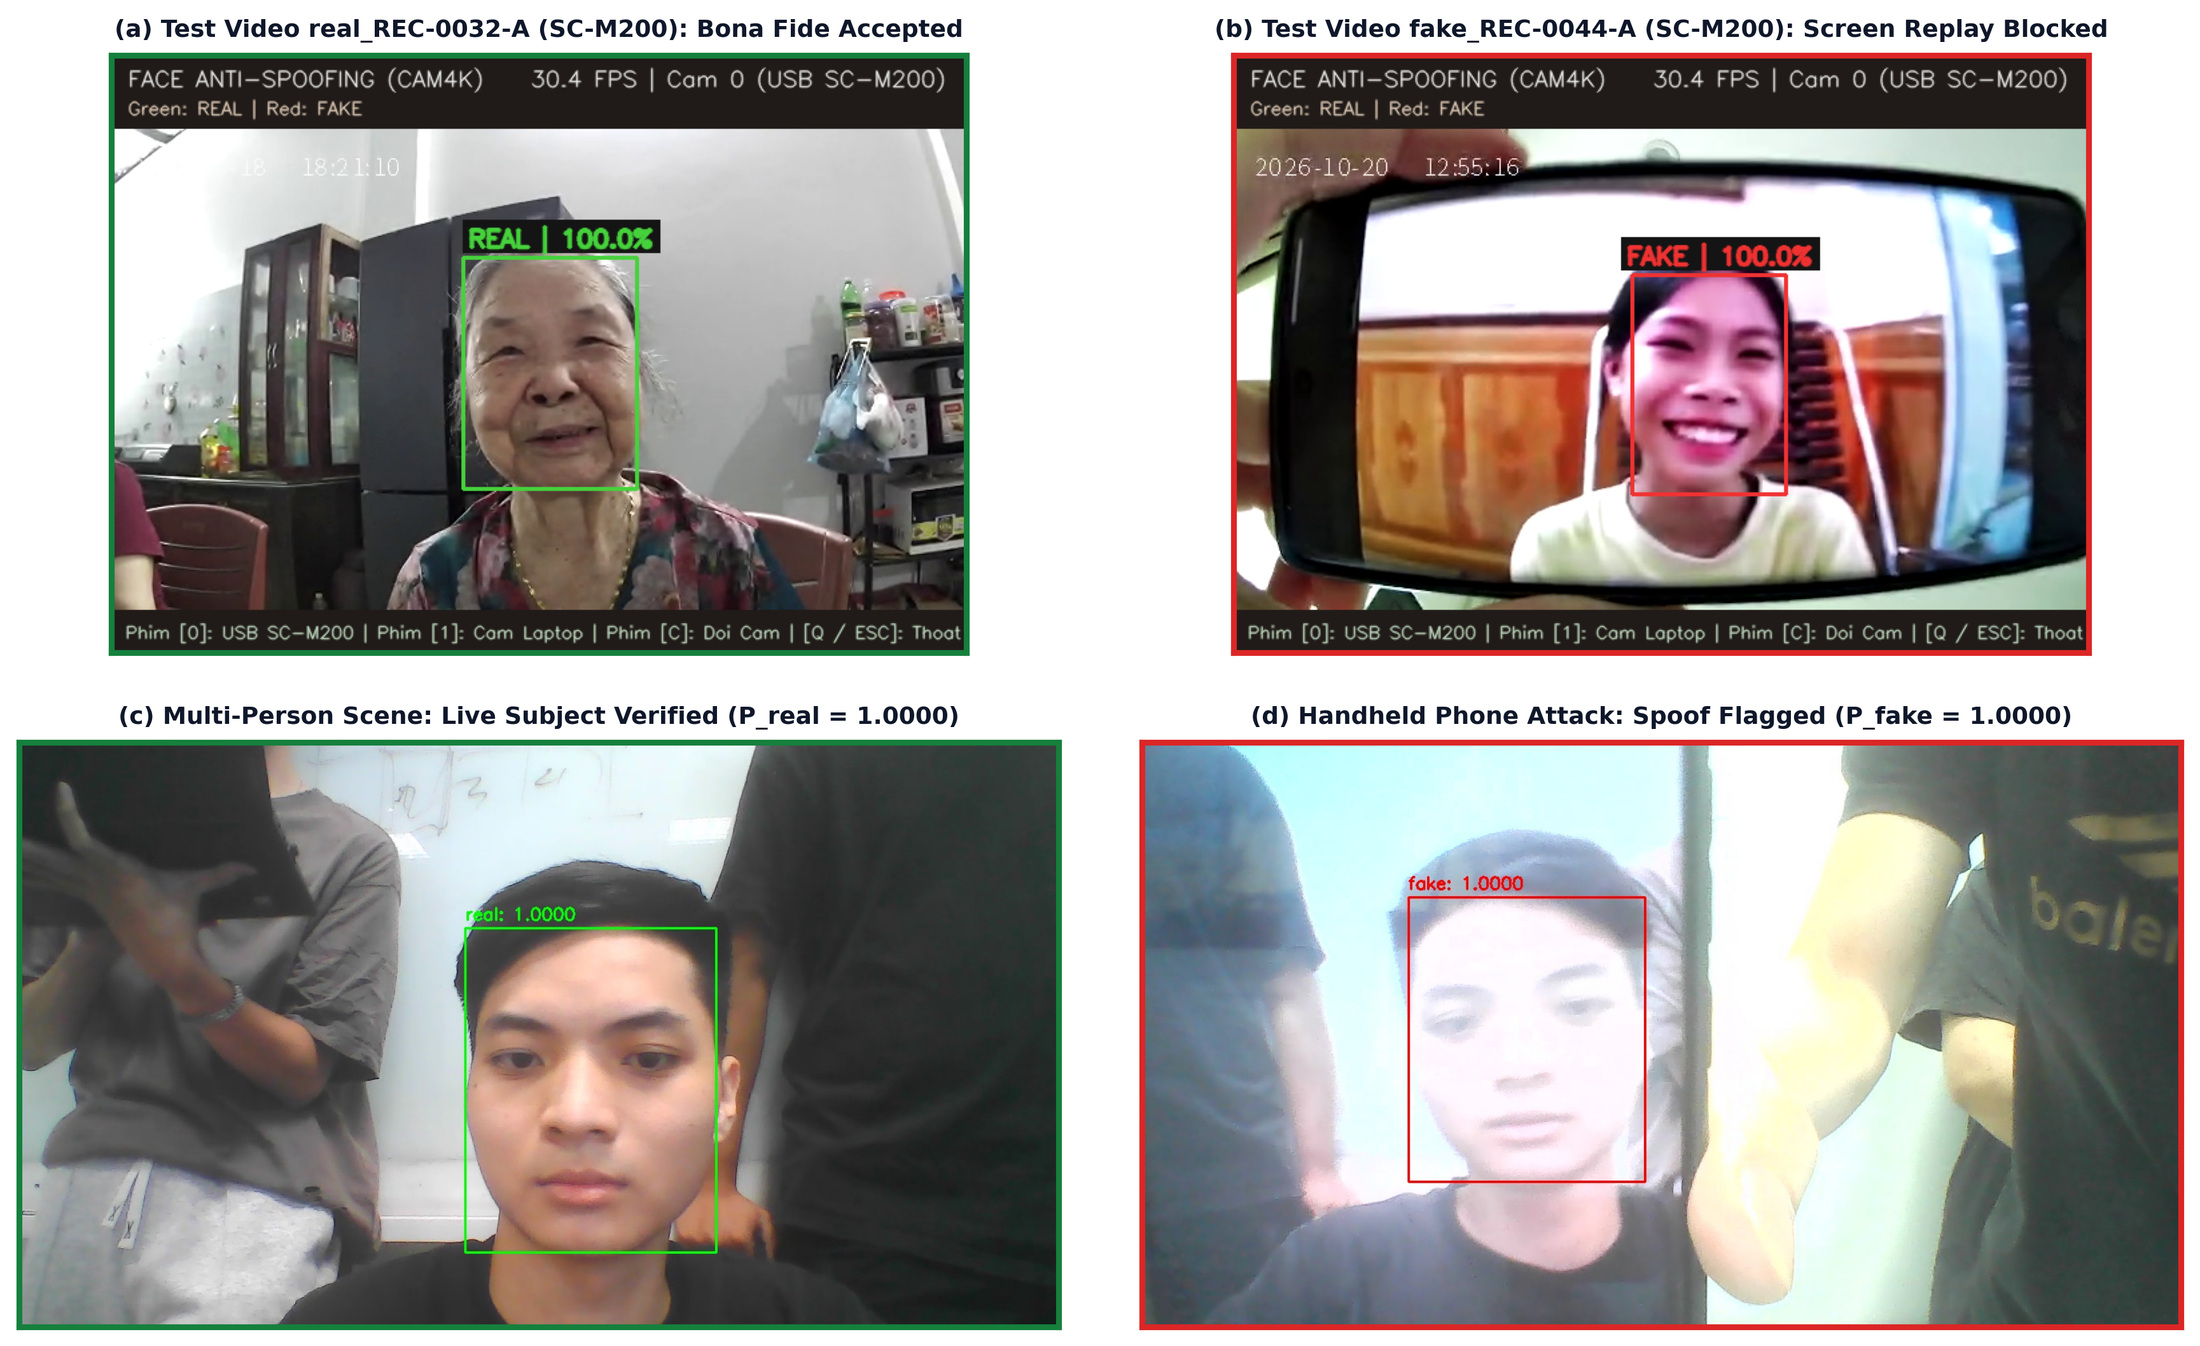
\includegraphics[width=0.98\textwidth]{Images/fig_qualitative_outputs.jpg}
\caption{Qualitative pipeline outputs across target SC-M200 test streams and indoor check-in scenes: (a) bona fide test subject accepted at $30.4$~FPS; (b) smartphone replay attack rejected with $100.0\%$ confidence; (c) foreground employee verified in a cluttered multi-person room; (d) high-glare handheld phone spoof flagged immediately.}
\label{fig:qualitative_results}
\end{figure}

In Figure~\ref{fig:qualitative_results}(a), an unseen elderly subject from \texttt{real\_REC-0032-A} is localized accurately by YuNet under cluttered domestic lighting and classified as \texttt{REAL | 100.0\%} at $30.4$~FPS without bounding-box jitter. In Figure~\ref{fig:qualitative_results}(b), a high-brightness landscape smartphone replay (\texttt{fake\_REC-0044-A}) is isolated inside the phone bezel and rejected at \texttt{FAKE | 100.0\%}, demonstrating that \texttt{LivenessNet} detects screen emission cues strictly from the internal $32\times32$ facial crop even when the surrounding hand and phone frame lie outside the classifier ROI. Figure~\ref{fig:qualitative_results}(c) and~(d) confirm consistent behavior in multi-person scenes where bystanders stand directly behind the primary subject: foreground live skin receives $P_{\text{real}} = 1.0000$, while an overexposed handheld display receives $P_{\text{fake}} = 1.0000$. Furthermore, recency-weighted \texttt{FastBinaryDecision} prevented transient label oscillation during natural blinking and speaking across all live camera trials.

\section{Error Analysis and Discussion}
\label{sec:error_analysis}

Rigorous inspection of the $92$ misclassified frames out of $4{,}811$ on the \texttt{Cam4K} test partition ($89$ false accepts and $3$ false rejects) reveals clear physical causes and architectural boundaries:
\begin{enumerate}
    \item \textbf{Concentration of false accepts in \texttt{fake\_REC-0041-A}:} Tracing the $89$ false-accept crops across Table~\ref{tab:video_breakdown} shows that the majority originate from a single recording, \texttt{fake\_REC-0041-A} (mean $P_{\text{real}} = 24.59\%$), with smaller clusters in \texttt{fake\_REC-0040-A} ($6.93\%$). Inspection of raw frames in \texttt{fake\_REC-0041-A} indicates that a high-pixel-density OLED phone was held at an intermediate distance ($\approx 0.65$~m) where camera sensor sampling fell below the subpixel Nyquist aliasing frequency, while screen brightness closely matched ambient room walls without overhead lamp reflections. Even under this worst-case optical alignment, $>75\%$ of frames in the clip still scored as \texttt{fake}, allowing temporal aggregation to reject the video cleanly.
    \item \textbf{Transient motion blur on bona fide frames:} All $3$ false-reject frames ($\text{BPCER} = 0.12\%$) occurred during rapid mid-clip head rotation where motion blur smeared skin pore micro-texture while overhead fluorescent lighting created a brief forehead highlight. Within $0.15$~seconds ($4$--$5$ frames), \texttt{FastBinaryDecision} recovered stable \texttt{real} output.
    \item \textbf{Lessons from container and detector domain shifts:} Earlier experiments between Cohort~I and Cohort~II demonstrated that mixing \texttt{.mov} and \texttt{.mp4} recordings or evaluating SCRFD face crops directly with an SSD-trained classifier degraded calibration significantly. Standardizing acquisition on the SC-M200 sensor in Cohort~III and introducing padded YuNet ROI re-alignment inside \texttt{LivenessGate} eliminated both failure modes.
    \item \textbf{Residual boundary on matte prints and extreme pose:} Because \texttt{Cam4K} focuses primarily on electronic display attacks, high-resolution matte inkjet photographs lacking specular glass glare represent a harder out-of-distribution case for pure CNN activations; enabling the optical $YC_rC_b$/HSV print-shield (\texttt{fusion=True}) mitigates desaturated paper veils, though dedicated multi-printer training corpora remain advisable for high-security print environments.
\end{enumerate}

\section{Comparison with Existing Works}
\label{sec:comparison_existing}

Table~\ref{tab:comparison_sota} situates the proposed system alongside representative passive RGB anti-spoofing methods from the literature and sequential project baselines. Because published PAD benchmarks differ in sensor resolution, attack instruments, and evaluation protocols (e.g., OULU-NPU Protocol~1~\cite{boulkenafet2017oulu} vs.\ SiW~\cite{liu2018learning} vs.\ person-disjoint \texttt{Cam4K}), literature metrics are cited under their native intra-dataset protocols to provide architectural context rather than direct cross-dataset ranking, whereas the bottom four rows compare progressive baselines strictly within this project's audited benchmarks.

\begin{table}[htbp]
\centering
\caption{Architectural and empirical comparison with representative passive RGB PAD methods and sequential project baselines.}
\label{tab:comparison_sota}
\small
\begin{tabular}{L{3.5cm}L{2.4cm}R{1.5cm}R{1.5cm}L{4.4cm}}
\toprule
\textbf{Method / Baseline} & \textbf{Dataset / Protocol} & \textbf{Params} & \textbf{ACER (\%)} & \textbf{Runtime \& Deployment Notes} \\
\midrule
LBP + SVM~\cite{chingovska2012effectiveness} & Replay-Attack & --- & $13.8$--$15.1$ & Fast CPU; brittle under AWB/OLED shifts. \\
Colour-LBP~\cite{boulkenafet2016face} & Replay / CASIA & --- & $2.8$--$7.1$ & Handcrafted $YC_bC_r$+HSV; no temporal tracker. \\
Aux-Depth CNN~\cite{liu2018learning} & OULU-NPU P1 & $>2.5\text{M}$ & $1.6$ & Requires pseudo-depth + rPPG GPU supervision. \\
CDCN~\cite{yu2020searching} & OULU-NPU P1 & $\approx 2.3\text{M}$ & $1.0$ & Central diff.\ convs; multi-ms CPU cost. \\
PatchNet~\cite{wang2022patchnet} & OULU-NPU P1 & $\approx 11.2\text{M}$ & $0.8$ & ResNet-18 backbone; GPU-oriented inference. \\
\midrule
Phase~1: Legacy Disjoint & Unseen Cohort~IIa & $0.55\text{M}$ & $26.39$ & $96.86\%$ in-domain, collapsed cross-subject. \\
Phase~2: Quality Retrain & Cohort~IIa Test & $0.55\text{M}$ & $2.29$ & $16/16$ video acc.; $-10.36$~pp legacy forgetting. \\
Phase~3: Stratified + GN & Merged $89$-Vid Test & $0.54\text{M}$ & $4.82$ & Solved BN drift; $0$ wrong in $942$-f replay. \\
\textbf{Phase~4: Proposed Aligned \texttt{LivenessNet}} & \textbf{\texttt{Cam4K} Disjoint Test} & $\mathbf{0.55\text{M}}$ & $\mathbf{1.94}$ & \textbf{$0.163$~ms CPU LiteRT; $14/14$ ($100\%$) video acc.; $99.84\%$ cross-cam.} \\
\bottomrule
\end{tabular}
\end{table}

Table~\ref{tab:comparison_sota} demonstrates that the proposed aligned \texttt{LivenessNet} achieves an $\text{ACER}$ ($1.94\%$) competitive with substantially heavier deep architectures ($2.3\text{M}$--$11.2\text{M}$ parameters) while using $4\times$--$20\times$ fewer parameters ($0.55\text{M}$) and executing in $0.163$~ms on a commodity CPU.

\section{Ablation Studies}
\label{sec:ablation_studies}

To isolate the exact contribution of each methodological component introduced in Chapters~\ref{chap:data_processing} and~\ref{chap:methodology}, three controlled ablation experiments were conducted. Figure~\ref{fig:ablation_latency} visualizes the progressive error reduction across training/normalization regimes alongside the CPU latency breakdown, and Table~\ref{tab:ablation} reports detailed numerical outcomes.

\begin{figure}[htbp]
\centering
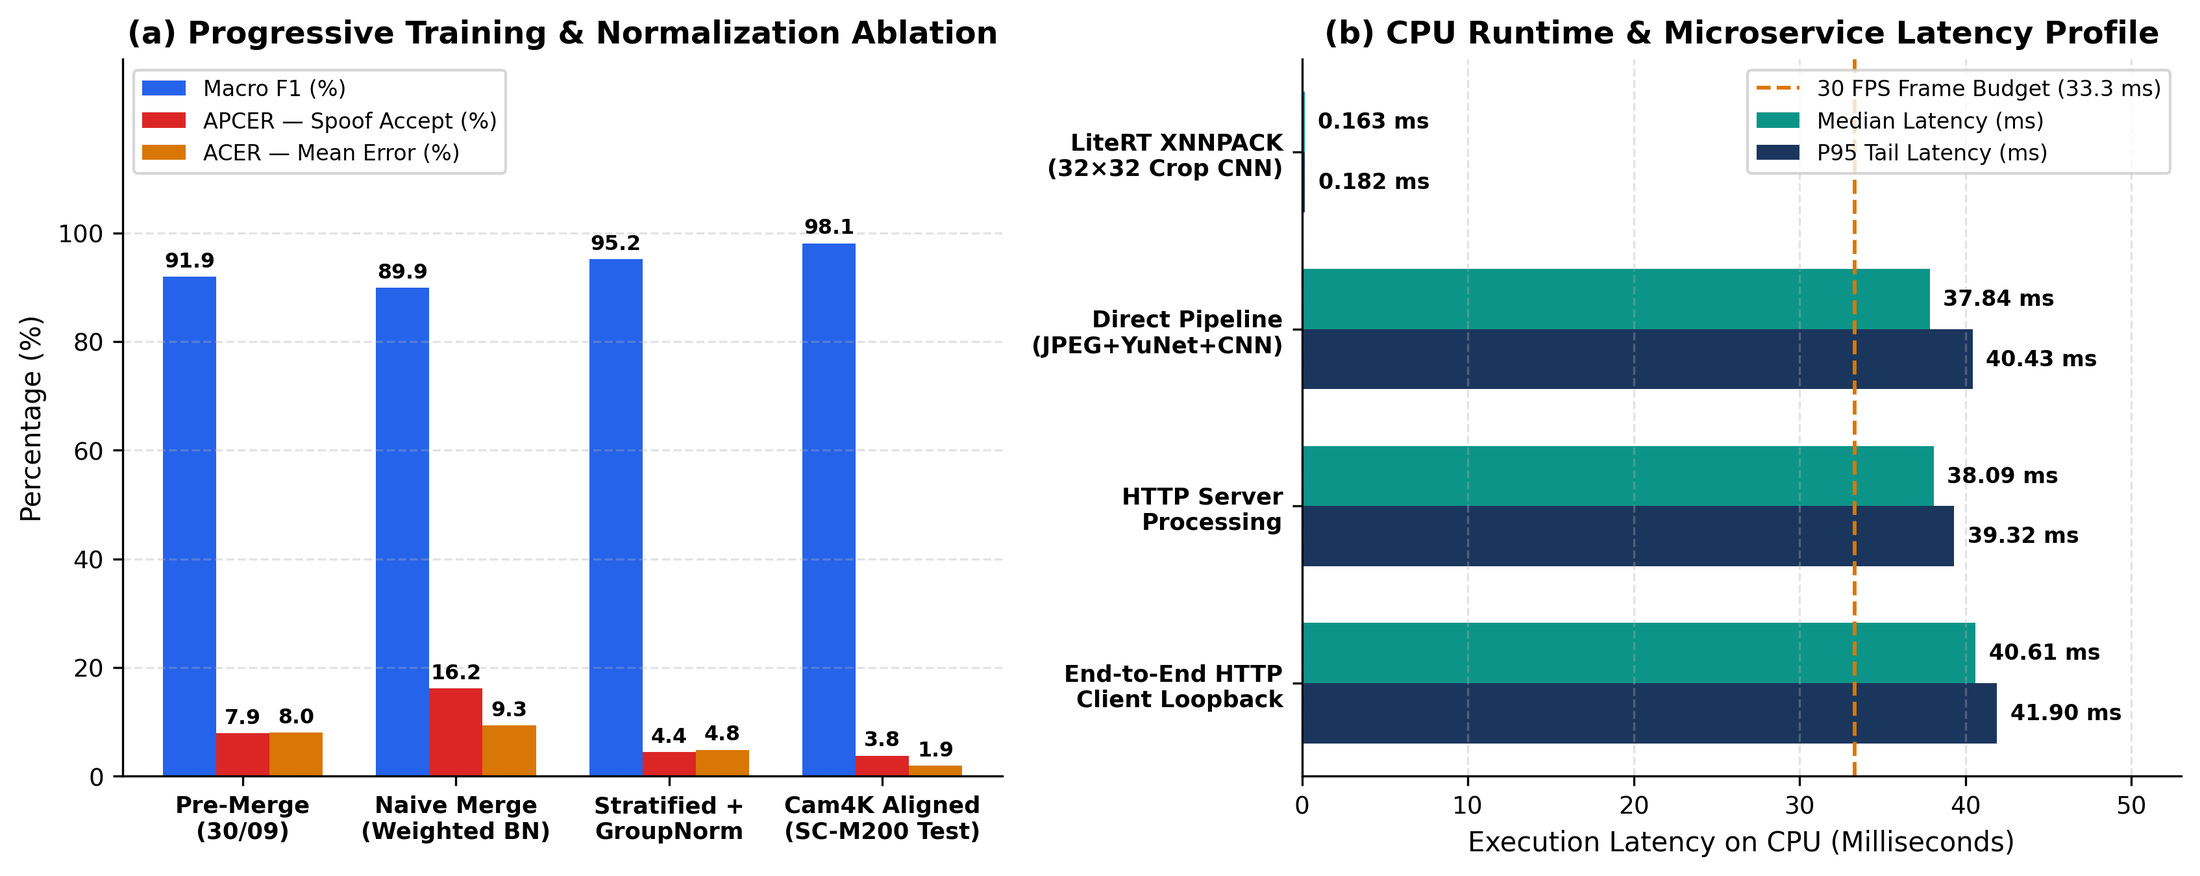
\includegraphics[width=0.98\textwidth]{Images/fig_ablation_and_latency.jpg}
\caption{Controlled ablation and runtime analysis: (a) Macro-$F_1$, $\text{APCER}$, and $\text{ACER}$ across progressive sampling and normalization configurations; (b) median and P95 CPU execution latency relative to the $33.3$~ms ($30$~FPS) real-time budget.}
\label{fig:ablation_latency}
\end{figure}

\begin{table}[htbp]
\centering
\caption{Multi-factor ablation results across normalization/sampling schemes, temporal aggregation policies, and CPU runtimes.}
\label{tab:ablation}
\small
\begin{tabular}{L{5.1cm}L{2.3cm}R{1.35cm}R{1.45cm}R{1.35cm}R{1.35cm}}
\toprule
\textbf{Ablation Configuration} & \textbf{Eval Benchmark} & \textbf{Acc (\%)} & \textbf{Macro $F_1$} & \textbf{APCER} & \textbf{ACER} \\
\midrule
\multicolumn{6}{l}{\emph{Factor A: Multi-Source Sampling \& Feature Normalization ($28{,}957$-crop Merged Corpus)}} \\
A1. Pre-Merge Baseline (Cohort~IIa only) & Merged Test ($4{,}856$) & $91.97$ & $91.90$ & $7.88$ & $8.03$ \\
A2. Naive Uniform Batch + Loss Weights + BN & Merged Test ($4{,}856$) & $89.99$ & $89.88$ & $16.16$ & $9.34$ \\
A3. Stratified $4\times8$ Queue + BatchNorm & Merged Val (Hier.) & \multicolumn{4}{r}{$\mathcal{L}_{\text{hier-val}} = 0.08422$ (vs.\ $0.26063$ post-hoc BN)} \\
A4. Stratified $4\times8$ + \texttt{GroupNorm}/\texttt{LayerNorm} & Merged Test ($4{,}856$) & $\mathbf{95.22}$ & $\mathbf{95.16}$ & $\mathbf{4.44}$ & $\mathbf{4.82}$ \\
\midrule
\multicolumn{6}{l}{\emph{Factor B: Temporal Decision Policy \& WiSE-FT Transfer}} \\
B1. Single-Frame Argmax ($\Delta_w = 1$ frame) & \texttt{Cam4K} Test ($4{,}811$) & $98.09$ & $98.09$ & $3.76$ & $1.94$ \\
B2. Video-Level Mean Score Aggregation & \texttt{Cam4K} Test ($14$ vids) & $\mathbf{100.00}$ & $\mathbf{100.00}$ & $\mathbf{0.00}$ & $\mathbf{0.00}$ \\
B3. Pre-Retrain Pipeline Session ($942$ frames) & Cohort~IIa $12$~s Replay & \multicolumn{4}{r}{$484$ correct, $173$ wrong ($26.3\%$ committed err.)} \\
B4. Retrained + \texttt{TemporalDecision} ($942$ frames) & Cohort~IIa $12$~s Replay & \multicolumn{4}{r}{$\mathbf{741}$ correct, $\mathbf{0}$ wrong ($\mathbf{0.0\%}$ err., $78.66\%$ cov.)} \\
\midrule
\multicolumn{6}{l}{\emph{Factor C: CPU Inference Graph Compilation ($32\times32\times3$ \texttt{float32} input)}} \\
C1. Keras~3 Eager \texttt{model.predict()} & Ryzen~7 6800H CPU & \multicolumn{4}{r}{$\approx 32.4\text{ ms}$ median per call ($1\times$ baseline)} \\
C2. Frozen LiteRT + XNNPACK (\texttt{LiteModel}) & Ryzen~7 6800H CPU & \multicolumn{4}{r}{$\mathbf{0.163\text{ ms}}$ median per call ($\mathbf{198\times}$ speedup)} \\
\bottomrule
\end{tabular}
\end{table}

Three key engineering insights emerge from Table~\ref{tab:ablation}:
\begin{enumerate}
    \item \textbf{Why naive weighted merging fails (A1--A4):} In Configuration~A2, uniform mini-batches drew $88.36\%$ legacy frames while scalar sample weights assigned $54.77\%$ of gradient magnitude to minority Cohort~II frames (maximum weight ratio $52.75\times$). Confirming the mathematical analysis in Equations~\eqref{eq:batchnorm}--\eqref{eq:bn_ema}, unweighted BatchNorm EMA statistics drifted away from the loss-weighted feature representations, causing $\text{APCER}$ to more than double from $7.88\%$ ($213/2704$) to $16.16\%$ ($437/2704$). Attempting post-hoc BN moving-statistic recalibration without retraining worsened hierarchical validation loss to $0.26063$, proving internal filter co-adaptation had already occurred. Enforcing exact $4\times8$ round-robin mini-batch stratification with unweighted gradients and sample-local \texttt{GroupNorm}/\texttt{LayerNorm} (A4) lowered $\mathcal{L}_{\text{hier-val}}$ to $0.07089$, cut $\text{APCER}$ by nearly fourfold ($16.16\% \to 4.44\%$), and restored legacy regression accuracy from $80.24\%$ to $91.33\%$.
    \item \textbf{Value of multi-frame temporal aggregation (B1--B4):} Aggregating frame probabilities across video tracks eliminates the $3.76\%$ single-frame spoof tail on \texttt{Cam4K} ($100.00\%$ video accuracy). Similarly, in continuous $12$-second real-time session replay across $16$ unseen videos ($942$ frames; paired bootstrap $95\%$ CI on video $F_1$ gain: $[+6.27, +54.11]$~percentage points), pairing the retrained network with \texttt{TemporalDecision} hysteresis completely eliminated all $173$ false session verdicts ($0$ wrong committed decisions across $741$ active predictions, $78.66\%$ coverage; and $714$ correct, $0$ wrong, $75.80\%$ coverage on the Phase~3 merged model).
    \item \textbf{Impact of static graph compilation (C1--C2):} Freezing \texttt{LivenessNet} into an XNNPACK-accelerated LiteRT flatbuffer achieved bit-identical floating-point predictions while accelerating CNN execution nearly two hundredfold ($32.4$~ms $\to 0.163$~ms), enabling concurrent YuNet detection, ArcFace recognition, and anti-spoofing on standard office CPUs.
\end{enumerate}
